\chapter{Local Times of Semimartingales}

Throughout, $(\Omega, \mathcal{F}, (\mathcal{F}_t)_{t\geqslant 0}, \mathbb{P})$
is a filtered probability space satisfying the usual conditions of right
continuity and completeness. Every continuous semimartingale $X$ is written
$X = X_0 + M + A$, where $M$ is a continuous local martingale and $A$ a
continuous adapted process of finite variation, with $M_0 = A_0 = 0$; we
denote by $|A|$ the total variation process of $A$. The presentation of this
chapter follows \citet{Durrett1996} and \citet[Chapter~VI]{RevuzYor1999}.

\section{Definition and First Properties}

In this section we prove an extension of It\^o's formula due to
\citet{Tanaka1963} and \citet{Meyer1976}: It\^o's formula remains valid, in a
modified form, when $f$ is a difference of two convex functions. It\^o's
formula tells us how $C^2$ functions act on continuous semimartingales; we
now extend this to convex functions, which leads to the important notion of
local time.

For a convex function $f:\mathbb{R}\to\mathbb{R}$, the left derivative
\[
	f'_-(x) = \lim_{h\downarrow 0} \frac{f(x)-f(x-h)}{h}
\]
exists at every $x$, and $f'_-$ is increasing and left continuous. Unless
stated otherwise, $f'$ denotes the left derivative $f'_-$.

\begin{theorem}\label{th1}
	Let $f:\mathbb{R}\to\mathbb{R}$ be a convex function and let $X$ be a
	continuous semimartingale. Then $f(X)$ is a semimartingale and there
	exists a continuous adapted increasing process $K^f$, with $K^f_0 = 0$,
	such that
	\[
		f(X_t)-f(X_0)=\int_0^t f'_-(X_s)\,dX_s +\frac{1}{2} K_t^f .
	\]
\end{theorem}

\begin{proof}
	Assume first that $|X_0| + |M_t| + |A|_t \leqslant N$ and
	$\langle M\rangle _t\leqslant N$ for all $t\geqslant 0$; in particular
	$|X_t|\leqslant N$.

	Let $g$ be a nonnegative $C^\infty$ function with compact support in
	$(-\infty,0]$ such that $\int_\mathbb{R} g(y)\,dy = 1$, and set
	\begin{equation}\label{eq1}
		f_n(x)=\int_\mathbb{R} f\Big(x+\frac{y}{n}\Big)g(y)\,dy .
	\end{equation}
	Then $f_n$ is convex and $C^\infty$, and It\^o's formula gives
	\begin{equation}\label{eq2}
		f_n(X_t)-f_n(X_0)=\int_0^t f_n'(X_s)\,dX_s + \frac{1}{2} K^n_t,
		\qquad
		K^n_t = \int_0^t f''_n(X_s)\,d\langle X\rangle _s .
	\end{equation}
	Our strategy is to let $n\to \infty$ in \eqref{eq2}. A convex function is
	Lipschitz continuous on bounded intervals, so $f_n\to f$ uniformly on
	compact sets and, since $|X_t| \leqslant N$,
	\begin{equation}\label{eq3}
		\sup_t |f_n(X_t) - f(X_t)| \longrightarrow 0 .
	\end{equation}
	For the stochastic integral, differentiating \eqref{eq1} gives
	\begin{equation}\label{eq4}
		f_n'(x)=\int_\mathbb{R} f'_-\Big( x+\frac{y}{n} \Big) g(y)\,dy
		\ \uparrow\ f'_-(x) \qquad (n\to\infty),
	\end{equation}
	because $y\leqslant 0$ on the support of $g$ and $f'_-$ is increasing and
	left continuous. Moreover $|f'_n|$ and $|f'_-|$ are bounded on $[-N,N]$
	by a constant $C_N$. Let
	\[
		I_t^n=\int_0^t f_n'(X_s)\,dM_s, \qquad I_t=\int_0^t f'_-(X_s)\,dM_s .
	\]
	Doob's $L^2$ maximal inequality and the isometry property of
	stochastic integrals give
	\[
		\E \Big( \sup_t (I_t^n-I_t)^2 \Big)
		\leqslant 4 \sup_t \E(I_t^n-I_t)^2
		= 4 \E\int_0^\infty (f_n'(X_s)- f'_-(X_s))^2\, d\langle M \rangle_s
		\longrightarrow 0
	\]
	by the bounded convergence theorem (recall that
	$\langle M\rangle_\infty \leqslant N$). Passing to a subsequence $(n_k)$,
	\begin{equation}\label{eq5}
		\sup_t |I_t^{n_k}-I_t| \longrightarrow 0\quad \text{almost surely.}
	\end{equation}
	For the finite variation part, let
	\[
		J_t^n=\int_0^t f_n'(X_s)\,dA_s, \qquad J_t=\int_0^t f'_-(X_s)\,dA_s ;
	\]
	by the bounded convergence theorem, for almost every $\omega$,
	\begin{equation}\label{eq6}
		\sup_t|J_t^n-J_t| \leqslant \int_0^\infty | f_n'(X_s)- f'_-(X_s)|\,
		d|A|_s\longrightarrow 0 .
	\end{equation}
	Finally, \eqref{eq2} can be rewritten as
	\begin{equation}\label{eq7}
		K_t^{n_k} = 2\Big(f_{n_k}(X_t)-f_{n_k}(X_0)
		-\int_0^t f'_{n_k}(X_s)\,dX_s \Big) .
	\end{equation}
	By \eqref{eq3}, \eqref{eq5} and \eqref{eq6}, the right-hand side of
	\eqref{eq7} converges almost surely, uniformly in $t$, to
	$2\big(f(X_t) - f(X_0) - \int_0^t f'_-(X_s)\,dX_s\big)$. Hence so does the
	left-hand side; as each $K^{n_k}$ is continuous, adapted and increasing,
	the limit $K^f$ is continuous, adapted and increasing, and the formula
	holds.

	In the general case, let
	$T_m=\inf \{ t\geqslant 0 : |X_0| + |M_t| + |A|_t + \langle M\rangle_t
	\geqslant m \}$ on $\{|X_0| < m\}$. Applying the first part to the stopped
	process $X^{T_m}$ on $\{|X_0|<m\}$ gives increasing processes $K^{f,m}$ such
	that
	\[
		f(X_{t\wedge T_m})=f(X_0)+\int_0^{t\wedge T_m} f'_-(X_s)\, dX_s
		+\frac{1}{2} K_t^{f,m} .
	\]
	By uniqueness of the limit, $K^{f,m+1}_t = K^{f,m}_t$ for $t\leqslant T_m$,
	so $K^f_t = K^{f,m}_t$ for $t\leqslant T_m$ defines a continuous adapted
	increasing process. Since $T_m \uparrow \infty$ and
	$\{|X_0|<m\}\uparrow\Omega$, the formula holds for all $t$.
\end{proof}

Since $f(X_t) - f(X_0) - \int_0^t f'_-(X_s)\,dX_s$ is determined by $f$ and
$X$, the process $K^f$ is unique, and $f \mapsto K^f$ is linear. If we fix
$X$, we call $K^f$ \textbf{the increasing process associated with} $f$. If
$f$ is affine, then $f(X_t) - f(X_0) = \int_0^t f'(X_s)\,dX_s$ and so
$K^f = 0$.

\begin{lemma}\label{lem:pm}
	For $a\in\mathbb{R}$, the increasing processes associated with $(x-a)^+$
	and with $(x-a)^-$ are equal. The increasing process associated with
	$|x-a|$ is twice this common process.
\end{lemma}

\begin{proof}
	Let $K^+$ and $K^-$ be the increasing processes associated with
	$(x-a)^+$ and $(x-a)^-$. Since $(x-a)^+ - (x-a)^- = x-a$ is affine,
	linearity gives $K^+ - K^- = K^{x-a} = 0$. Since
	$|x-a| = (x-a)^+ + (x-a)^-$, the process associated with $|x-a|$ is
	$K^+ + K^- = 2K^+$.
\end{proof}

\begin{definition}\label{def:localtime}
	The increasing process associated with $(x-a)^+$ is called the
	\textbf{local time of $X$ at $a$} and is denoted by $L^a = (L^a_t)_{t\geqslant 0}$.
	We write $L^a(X)$ when there is a risk of ambiguity.
\end{definition}

We define the function $\sgn$ by $\sgn(x)=1$ if $x>0$ and $\sgn(x)=-1$ if
$x\leqslant 0$, so that the left derivative of $|x|$ is $\sgn(x)$.

\subsection{Tanaka's formula}

\begin{theorem}[Tanaka's formula]\label{th:tanaka}
	Let $X$ be a continuous semimartingale. For every $a\in\mathbb{R}$, the
	local time $L^a$ is a continuous increasing process and
	\begin{align*}
		|X_t - a|      & =|X_0 - a| + \int_0^t \sgn( X_s - a)\,dX_s + L_t^a,                                \\
		(X_t - a)^{+} & =(X_0 - a)^{+}+ \int_0^t 1_{\{X_s > a\}}\, dX_s + \frac{1}{2} L_t^a,        \\
		(X_t - a)^{-} & =(X_0 - a)^{-}- \int_0^t 1_{\{X_s \leqslant a\}}\, dX_s + \frac{1}{2} L_t^a.
	\end{align*}
	In particular $|X-a|$, $(X-a)^+$ and $(X-a)^-$ are semimartingales.
\end{theorem}

\begin{proof}
	The left derivatives of $(x-a)^+$, $(x-a)^-$ and $|x-a|$ are
	$1_{]a,\infty[}(x)$, $-1_{]-\infty,a]}(x)$ and $\sgn(x-a)$. The three
	formulas follow from Theorem~\ref{th1} and Lemma~\ref{lem:pm}.
\end{proof}

\begin{remark}
	The lack of symmetry between the last two identities comes from the
	choice of left derivatives, which also dictates the convention
	$\sgn(0) = -1$.
\end{remark}

\begin{remark}
	The increasing process $L^a$ defines a random Stieltjes measure
	$dL_t^a$ on $\mathbb{R}_+$. It measures the ``time'' spent at $a$ by the
	semimartingale $X$, as the following results show.
\end{remark}

\begin{theorem}\label{th3}
	The local time $L^a$ only increases when $X = a$: almost surely, the
	measure $dL^a_t$ is carried by the set $\{ t\geqslant 0 : X_t = a\}$, that is
	\[
		\int_0^\infty 1_{\{X_s \neq a\}}\, dL^a_s = 0 .
	\]
\end{theorem}

\begin{proof}
	The process $Y = |X-a|$ is a semimartingale with
	$dY_s = \sgn(X_s - a)\,dX_s + dL^a_s$ and $\langle Y\rangle = \langle X\rangle$.
	It\^o's formula applied to $Y^2 = (X-a)^2$ gives
	\[
		(X_t - a)^{2} =(X_0 - a)^{2}+ 2 \int_0^t |X_s - a| \sgn(X_s -a)\,dX_s
		+ 2 \int_0^t |X_s - a|\,dL_s^a + \langle X \rangle _t,
	\]
	while It\^o's formula applied directly to $(X-a)^2$ gives
	\[
		(X_t - a)^{2} =(X_0 - a)^{2}+ 2 \int_0^t (X_s - a )\,dX_s+ \langle X \rangle _t .
	\]
	Since $|x-a|\sgn(x-a) = x-a$, comparing the two identities yields
	$\int_0^t |X_s - a|\,dL_s^a=0$ for all $t$, almost surely, which is the claim.
\end{proof}

\begin{remark}
	It is natural to ask whether $\{ t : X_t =a \}$ is exactly the support
	of $dL^a_t$. This is not true in general, but it is true for Brownian
	motion \citep[Chapter~VI]{RevuzYor1999}.
\end{remark}

We are now ready for the main result of this section.

\subsection{It\^o--Tanaka formula}

\begin{theorem}[It\^o--Tanaka formula]\label{th4}
	Let $X$ be a continuous semimartingale and let $f$ be the difference of
	two convex functions, with left derivative $f'_-$ and second derivative
	$f''=\mu$ in the sense of distributions (that is, $\mu$ is the signed
	measure such that $\mu(]x,y]) = f'_-(y+) - f'_-(x+)$). Then
	\[
		f(X_t)-f(X_0)=\int_0^t f'_-(X_s)\,dX_s + \frac{1}{2}\int_\mathbb{R} L_t^a \,\mu(da) .
	\]
	In particular, $f(X)$ is a semimartingale.
\end{theorem}

\begin{proof}
	The formula is linear in $f$, so we may assume that $f$ is convex and
	$\mu$ is a positive measure. By stopping, we may assume that
	$|X_t| \leqslant N$ and $\langle X\rangle _t \leqslant N$ for all $t$.
	Let
	\[
		g(x)=\frac{1}{2}\int_{[-N,N]} |x-a|\,\mu(da) .
	\]
	Then $(f-g)''=0$ on $]-N,N[$ in the sense of distributions, so
	$f(x)-g(x)=\alpha+\beta x$ for $|x|\leqslant N$, and since the formula is
	trivial for affine functions, it suffices to prove it for $g$. The left
	derivative of $g$ is
	\[
		g'_-(x)=\frac{1}{2}\int_{[-N,N]} \sgn(x-a)\,\mu(da) .
	\]
	Integrating Tanaka's formula
	$|X_t - a| =|X_0 - a| + \int_0^t \sgn( X_s - a)\,dX_s + L_t^a$
	with respect to $\frac{1}{2}\mu(da)$ over $[-N,N]$ gives
	\[
		g(X_t)-g(X_0)= \frac{1}{2} \int_{[-N,N]} \Big(\int_0^t \sgn( X_s - a)\,dX_s\Big)\mu(da)
		+ \frac{1}{2} \int_{[-N,N]} L_t^a\, \mu(da) .
	\]
	Lemma~\ref{lem2} and Theorem~\ref{th5} below justify interchanging the
	two integrals in the first term, which gives
	\[
		g(X_t)-g(X_0)= \int_0^t g'_-(X_s)\,dX_s + \frac{1}{2} \int_{[-N,N]} L_t^a\,\mu(da) .
	\]
	Finally, for $|a| > N$ the process $X$ never visits $a$, so $L_t^a=0$ by
	Theorem~\ref{th3}. This proves the result for $g$ and completes the proof.
\end{proof}

For the next two results, let $(S,\mathcal{S})$ be a measurable space and
$\mu$ a finite measure on $(S,\mathcal{S})$. For our purpose it would be enough
to take $S=\mathbb{R}$, but it is just as easy to treat a general space. We
denote by $\mathcal{P}$ the predictable $\sigma$-field on
$\mathbb{R}_+\times\Omega$, that is, the smallest $\sigma$-field containing
all the sets $]s,u]\times B$ with $s<u$ and $B\in \mathcal{F}_s$, together
with the sets $\{0\}\times B$ with $B \in\mathcal{F}_0$.

The first step in justifying the interchange of the order of integration is a
measurability issue: given a family $H_t^a(\omega)$ of integrands indexed by
$a \in S$, we want to choose the integrals $\int_0^t H_s^a\,dX_s$ so that they
form a measurable function of $(a,t,\omega)$.

\begin{lemma}\label{lem2}
	Let $X$ be a continuous semimartingale and let
	$H_t^a(\omega)=H(a,t,\omega)$ be bounded and
	$\mathcal{S} \otimes \mathcal{P}$-measurable. Then there exists a
	$\mathcal{S} \otimes \mathcal{B}(\mathbb{R}_+)\otimes\mathcal{F}$-measurable
	function $Z(a,t,\omega)$ such that, for every $a\in S$,
	$(Z(a,t,\cdot))_{t\geqslant 0}$ is a continuous version of
	$\big(\int_0^t H_s^a\,dX_s\big)_{t\geqslant 0}$.
\end{lemma}

\begin{proof}
	By stopping, we may assume that $|A|_\infty \leqslant N$ and
	$\langle M\rangle_\infty \leqslant N$. Let $\mathcal{H}$ be the set of bounded
	$\mathcal{S}\otimes \mathcal{P}$-measurable $H$ for which the conclusion
	holds. We check the assumptions of the monotone class theorem (functional
	version).

	Clearly $\mathcal{H}$ is a vector space containing the constants. If
	$H(a,t,\omega)=f(a)K(t,\omega)$ where $f$ is bounded and
	$\mathcal{S}$-measurable and $K$ is bounded and $\mathcal{P}$-measurable, then
	$Z(a,t,\omega) = f(a)\,(K\cdot X)_t(\omega)$ is suitable, where
	$K\cdot X$ is a continuous version of $\int_0^\cdot K_s\,dX_s$. Hence
	$\mathcal{H}$ contains the indicators of the sets $C\times D$ with
	$C\in \mathcal{S}$ and $D\in\mathcal{P}$, which form a class closed under
	finite intersections and generating $\mathcal{S}\otimes\mathcal{P}$.

	Let now $H^n\in\mathcal{H}$ with $0\leqslant H^n \uparrow H$, $H$ bounded,
	and let $Z^n$ be the corresponding functions. For every $a$, Doob's $L^2$
	inequality, the isometry property and the bounded convergence theorem
	give
	\[
		\E\Big( \sup_t |(H^{n,a}\cdot M)_t-(H^{a}\cdot M)_t|^2 \Big)
		\leqslant 4\, \E\int_0^\infty (H^{n,a}_s - H^a_s)^2\, d\langle M \rangle_s
		\longrightarrow 0,
	\]
	and, for every $\omega$,
	$\sup_t |(H^{n,a}\cdot A)_t-(H^{a}\cdot A)_t| \leqslant
		\int_0^\infty |H^{n,a}_s - H^a_s|\,d|A|_s \to 0$. Thus, for every $a$,
	$Z^n(a,\cdot)$ converges to $H^a\cdot X$ uniformly in probability, and
	\[
		\rho_n(a) = \sup_{m \geqslant n}\E\Big[\sup_t |Z^n(a,t)-Z^m(a,t)| \wedge 1\Big]
		\longrightarrow 0 \qquad (n\to\infty).
	\]
	Each $\rho_n$ is $\mathcal{S}$-measurable by Fubini's theorem. Let
	$n_0(a)=0$ and $n_{k}(a) = \inf\{n > n_{k-1}(a) : \rho_n(a) \leqslant 2^{-k}\}$;
	these are $\mathcal{S}$-measurable, and
	$\E\big[\sup_t |Z^{n_k(a)}(a,t)-Z^{n_{k+1}(a)}(a,t)| \wedge 1\big]
		\leqslant 2^{-k}$. Hence, for every $a$, almost surely
	$\sum_k \sup_t |Z^{n_k(a)}(a,t)-Z^{n_{k+1}(a)}(a,t)|\wedge 1 < \infty$, and
	$Z^{n_k(a)}(a,\cdot)$ converges uniformly in $t$. Let $Z(a,t,\omega)$ be this
	limit where it exists and $0$ elsewhere. Since
	$Z^{n_k(a)}(a,t,\omega) = \sum_n 1_{\{n_k(a) = n\}} Z^n(a,t,\omega)$ is measurable,
	so is $Z$; it is continuous in $t$, and for every $a$ it is a version of
	$H^a\cdot X$. Thus $H\in\mathcal{H}$, and the monotone class theorem
	completes the proof.
\end{proof}

\begin{theorem}[Fubini's theorem for stochastic integrals]\label{th5}
	Let $X$ be a continuous semimartingale, let $H^a_t$ be bounded and
	$\mathcal{S}\otimes \mathcal{P}$-measurable, and let $Z^a_t = Z(a,t,\omega)$ be
	any measurable function such that, for every $a$, $Z^a$ is a continuous
	version of $\int_0^\cdot H_s^a\,dX_s$ (such a function exists by
	Lemma~\ref{lem2}).
	Then $H_t=\int_S H^a_t\,\mu(da)$ is predictable and bounded, and
	$Y_t=\int_S Z^a_t\,\mu(da)$ is a version of $\int_0^t H_s\,dX_s$. Less formally,
	\[
		\int_S \Big(\int_0^t H^a_s\,dX_s\Big) \mu(da)=\int_0^t\Big(\int_S H^a_s\,\mu(da)\Big)dX_s .
	\]
\end{theorem}

\begin{proof}
	The predictability of $H$ follows from the classical Fubini theorem. By
	stopping, we may assume that $|A|_\infty \leqslant N$ and
	$\langle M\rangle_\infty \leqslant N$. When $X=A$ the result is the
	classical Fubini theorem applied for each $\omega$, so we may assume that
	$X=M$. Let $\mathcal{H}$ be the set of bounded $\mathcal{S}\otimes
	\mathcal{P}$-measurable $H$ for which the conclusion holds; it is a vector
	space containing the constants.

	If $H(a,t,\omega)=f(a)K(t,\omega)$ with $f$ bounded and
	$\mathcal{S}$-measurable and $K$ bounded and $\mathcal{P}$-measurable, then
	$Z^a_t=f(a)(K\cdot M)_t$ and
	\[
		\int_S Z^a_t\,\mu(da) = \Big(\int_S f(a)\,\mu(da)\Big)(K\cdot M)_t
		= \Big( \Big(\int_S f(a)\,\mu(da)\Big) K\Big) \cdot M_t = (H\cdot M)_t,
	\]
	so $\mathcal{H}$ contains the indicators of the sets $C\times D$ with
	$C\in\mathcal{S}$ and $D\in\mathcal{P}$.

	Let now $H^n\in\mathcal{H}$ with $0\leqslant H^n \uparrow H$, $H$ bounded.
	Write $Z^{n,a}$ for the versions associated with $H^{n,a}$ and
	$H^n_t = \int_S H^{n,a}_t\,\mu(da)$. By the Cauchy--Schwarz inequality,
	Doob's $L^2$ inequality and the isometry property,
	\[
		\E \sup_t \Big|\int_S Z^{n,a}_t\,\mu(da) - \int_S Z^a_t\,\mu(da)\Big|
		\leqslant \int_S \Big( 4\,\E\int_0^\infty (H^{n,a}_s - H^a_s)^2\,
		d\langle M\rangle_s \Big)^{1/2} \mu(da) \longrightarrow 0
	\]
	by the bounded convergence theorem, used twice. On the other hand
	$H^n \uparrow H$ boundedly, so
	\[
		\E \sup_t |(H^n\cdot M)_t - (H\cdot M)_t|^2 \leqslant
		4\,\E\int_0^\infty (H^n_s - H_s)^2\,d\langle M\rangle_s \longrightarrow 0 .
	\]
	Since $\int_S Z^{n,a}_t\,\mu(da) = (H^n\cdot M)_t$ by assumption, the two
	limits agree: $\int_S Z^{a}_t\,\mu(da) = (H\cdot M)_t$ for all $t$, almost
	surely. Hence $H\in\mathcal{H}$, and the monotone class theorem completes
	the proof.
\end{proof}

We can now complete the identification of $L^a_t$ as the time spent at $a$.

\subsection{Occupation times formula}

\begin{theorem}[Occupation times formula]\label{th6}
	Let $X$ be a continuous semimartingale with local times $(L^a_t)$. Almost
	surely, for every $t \geqslant 0$ and every bounded Borel function
	$g:\mathbb{R}\to\mathbb{R}$,
	\[
		\int_\mathbb{R} L^a_t\, g(a)\,da=\int^t_0 g(X_s)\,d\langle X\rangle _s.
	\]
\end{theorem}

\begin{proof}
	Let $g$ be continuous and let $f\in C^2$ with $f''=g$. It\^o's formula
	gives
	\[
		f(X_t)-f(X_0)=\int_0^t f'(X_s)\,dX_s+\frac{1}{2}\int_0^t g(X_s)\,d\langle X\rangle_s,
	\]
	while the It\^o--Tanaka formula, with $\mu(da)=g(a)\,da$, gives
	\[
		f(X_t)-f(X_0)=\int_0^t f'(X_s)\,dX_s+\frac{1}{2}\int_\mathbb{R} L_t^a\, g(a)\,da .
	\]
	Comparing the two identities,
	$\int_\mathbb{R} L_t^a g(a)\,da=\int_0^t g(X_s)\,d\langle X\rangle_s$ for
	every continuous $g$, almost surely. Taking $g$ in a countable family of
	continuous functions with compact support that determines measures, we
	obtain that, almost surely and for every $t$, the two measures
	$L^a_t\,da$ and $A\mapsto \int_0^t 1_A(X_s)\,d\langle X\rangle_s$ coincide,
	which is the claim.
\end{proof}

\begin{remark}
	When $X$ is a Brownian motion, the identity in Theorem~\ref{th6} becomes
	\[
		\int_\mathbb{R} L^a_t\, g(a)\,da=\int^t_0 g(X_s)\,ds .
	\]
	Thus $L_t^a$ can be thought of as the time spent at $a$ up to time $t$:
	more precisely, $a\mapsto L^a_t$ is a density of the occupation measure
	$\nu_t(A)=\int_0^t 1_A(X_s)\,ds$ with respect to Lebesgue measure. For a
	general continuous semimartingale, the occupation measure is defined with
	respect to $d\langle X\rangle_s$, which may be seen as the ``natural'' time
	scale of $X$.
\end{remark}

There are many ways of defining the local time of Brownian motion. The one
given above has the advantage of making it easy to prove the existence of a
version in which $L^a_t$ is a jointly continuous function of $(a,t)$. This
property holds for every continuous local martingale, and it is no more
difficult to prove it in this generality.

\begin{theorem}\label{th7}
	Let $X$ be a continuous local martingale. There is a version of the
	family $(L^a_t)$ such that $(a,t)\mapsto L^a_t$ is continuous, almost surely.
\end{theorem}

\begin{proof}
	By stopping, we may assume that $|X_t| \leqslant N$ and
	$\langle X\rangle _t\leqslant N$ for all $t\geqslant 0$. By Tanaka's formula,
	\[
		\frac{1}{2}L^a_t=(X_t - a)^{+} -(X_0 - a)^{+}- \int_0^t 1_{\{X_s > a\}}\, dX_s .
	\]
	The map $(a,t)\mapsto (X_t - a)^{+} -(X_0 - a)^{+}$ is continuous, so it
	suffices to find a jointly continuous version of
	\[
		I_t^a = \int_0^t 1_{\{X_s > a\}}\, dX_s .
	\]
	Fix $T<\infty$ and regard $a\mapsto I^a$ as a random variable with values
	in $C([0,T],\mathbb{R})$, equipped with the norm
	$\|f\|_{\infty} =\sup_{0\leqslant t\leqslant T}|f(t)|$. By Kolmogorov's
	continuity theorem, it suffices to show that for some constants
	$\alpha, \beta, C>0$,
	\[
		\E\|I^a- I^b\|_\infty^\beta \leqslant C|a-b|^{1+\alpha}.
	\]
	Let $a<b$. Since $1_{\{X_s > a\}} - 1_{\{X_s > b\}} = 1_{\{a < X_s \leqslant b\}}$,
	the Burkholder--Davis--Gundy inequality, the occupation times formula and
	the Cauchy--Schwarz inequality give
	\begin{align*}
		\E\|I^a- I^b\|_\infty^4 & \leqslant C \E\Big(\int_0^T 1_{\{a< X_s \leqslant b\}}\, d\langle X\rangle_s\Big)^2
		= C\E\Big(\int_a^b L_T^x \, dx\Big)^2                                                                      \\
		                        & \leqslant C(b-a)\, \E\int_a^b (L_T^x)^2\, dx
		\leqslant C(b-a)^2 \sup_{x\in \mathbb{R}} \E(L_T^x)^2 .
	\end{align*}
	To bound the supremum, we use Tanaka's formula
	\[
		L_T^x = |X_T - x| - |X_0 - x| - \int_0^T \sgn( X_s - x)\,dX_s
	\]
	together with $(u+v)^2 \leqslant 2u^2 + 2v^2$ and
	$\big||y-x| -|z-x|\big|\leqslant |y-z|$:
	\[
		\E(L_T^x)^2 \leqslant 2 \E(X_T - X_0)^2 + 2\E\Big( \int_0^T \sgn(X_s-x)\, dX_s \Big)^2
		\leqslant 2(2N)^2 + 2\E\langle X \rangle_T \leqslant 8N^2+2N,
	\]
	by the isometry property and the bounds imposed by stopping. Hence
	$\E\|I^a- I^b\|_\infty^4 \leqslant C' (b-a)^2$, which is Kolmogorov's
	condition with $\beta = 4$ and $\alpha = 1$.
\end{proof}

\begin{example}[Reflected Brownian motion]
	Theorem~\ref{th7} fails for the semimartingale $X_t=|B_t|$, where $B$ is
	a Brownian motion. For $a>0$, $X$ visits $a$ exactly when $B$ visits $a$ or
	$-a$, and one checks that $L^a_t(X)=L^a_t(B)+ L^{-a}_t(B)$, while
	$L^a_t(X)=0$ for $a<0$. Since $L^0_t(B)> 0$ for $t>0$, the map
	$a\mapsto L^a_t(X)$ is discontinuous at $a=0$.

	This example is somewhat trivial since $0$ is an end point of the set of
	values of $X$. The skew Brownian motion, studied in
	Chapter~\ref{ch:sbm}, provides an example with $0$ in the interior.
\end{example}

We now construct the regular version of local times with which we work from
now on.

\begin{theorem}\label{th8}
	Let $X = X_0 + M + V$ be a continuous semimartingale. There exists a
	modification of the family $\{ L_t^a ; a\in \mathbb{R} , t\in \mathbb{R}_+ \}$
	such that, almost surely, $(a,t)\mapsto L_t^a$ is continuous in $t$ and
	càdlàg in $a$. Moreover, for every $a$,
	\[
		L_t^a - L_t^{a-} = 2\int_0^t 1_{\{X_s = a\}}\, dV_s=2\int_0^t 1_{\{X_s = a\}}\, dX_s .
	\]
	In particular, if $X$ is a local martingale, the family of local times
	has a bicontinuous modification.
\end{theorem}

\begin{proof}
	By Tanaka's formula,
	\[
		L_t^a =2\Big[(X_t - a)^{+} - (X_0 - a)^{+} - \int_0^t 1_{\{X_s > a\}}\, dM_s
		-\int_0^t 1_{\{X_s > a\}}\, dV_s \Big] .
	\]
	The argument of the proof of Theorem~\ref{th7} shows that
	$\widehat{M}_t^a = \int_0^t 1_{\{X_s > a\}}\, dM_s$ has a version which is
	jointly continuous in $(a,t)$: after stopping so that $|X|$,
	$\langle M\rangle$ and $|V|$ are bounded by $N$, the Burkholder--Davis--Gundy
	inequality and the occupation times formula (recall that
	$\langle X\rangle = \langle M\rangle$) give
	$\E\sup_{t\leqslant T}|\widehat{M}^a_t - \widehat{M}^b_t|^4 \leqslant C(b-a)^2\sup_x\E(L^x_T)^2$,
	and Tanaka's formula gives $\sup_x \E(L^x_T)^2 \leqslant 3(4N^2 + N + N^2)$.
	It remains to study
	\[
		\widehat{V}_t^a = \int_0^t 1_{\{X_s > a\}}\, dV_s ,
	\]
	which is continuous in $t$ for every $a$. By dominated convergence with
	respect to $|dV|$,
	\[
		\lim_{b\downarrow a}\widehat{V}_t^{b} = \int_0^t 1_{\{X_s > a \}}\, dV_s = \widehat{V}_t^{a},
		\qquad
		\lim_{b\uparrow a}\widehat{V}_t^{b} = \int_0^t 1_{\{X_s \geqslant a\}}\, dV_s ,
	\]
	so $a \mapsto \widehat{V}^a_t$ is càdlàg, and therefore so is
	$a\mapsto L^a_t$. Moreover
	\[
		L_t^a - L_t^{a-} =2\big( \widehat{V}_t^{a-} - \widehat{V}_t^{a}\big)
		=2\int_0^t 1_{\{X_s = a\}}\, dV_s .
	\]
	Finally, the occupation times formula gives
	\[
		\int_0^t 1_{\{X_s = a\}}\, d\langle M\rangle_s =
		\int_0^t 1_{\{X_s = a\}}\, d\langle X\rangle_s =
		\int_\mathbb{R} 1_{\{a\}}(x) L^x_t\, dx = 0,
	\]
	so the local martingale $\int_0^t 1_{\{X_s = a\}}\, dM_s$ has zero quadratic
	variation and vanishes. This gives the second equality.
\end{proof}

\begin{remark}
	If $X$ is a continuous process of finite variation, then $\langle X\rangle = 0$,
	so the occupation times formula gives $L^a(X) = 0$ for almost every $a$,
	hence for every $a$ by right continuity.
\end{remark}

From now on, we only consider the version of the local times given by
Theorem~\ref{th8}. For this version, the following corollary gives another
justification of the name ``local time''.

\begin{corollary}\label{cor1}
	If $X$ is a continuous semimartingale then, almost surely, for every $a$
	and $t$,
	\[
		L_t^a(X)=\lim_{\varepsilon \downarrow 0} \frac{1}{\varepsilon}
		\int_0^t 1_{[a,a+\varepsilon[}(X_s)\,d\langle X\rangle_s .
	\]
	If $M$ is a continuous local martingale, then almost surely, for every $a$
	and $t$,
	\[
		L_t^a(M)=\lim_{\varepsilon \downarrow 0} \frac{1}{2\varepsilon}
		\int_0^t 1_{]a-\varepsilon , a+\varepsilon[}(M_s)\,d\langle M\rangle_s .
	\]
\end{corollary}

\begin{proof}
	By the occupation times formula,
	\[
		\frac{1}{\varepsilon}\int_0^t 1_{[a,a+\varepsilon[}(X_s)\,d\langle X\rangle_s
		= \frac{1}{\varepsilon}\int_a^{a+\varepsilon} L^x_t\, dx,
	\]
	which converges to $L^a_t$ as $\varepsilon\downarrow 0$ by right continuity of
	$x\mapsto L^x_t$. For a continuous local martingale, $x\mapsto L^x_t$ is
	continuous by Theorem~\ref{th8}, and
	$\frac{1}{2\varepsilon}\int_{a-\varepsilon}^{a+\varepsilon} L^x_t\, dx \to L^a_t$.
\end{proof}

\begin{remark}
	For a Brownian motion $B$, we have in particular
	\[
		L_t^a(B)=\lim_{\varepsilon \downarrow 0} \frac{1}{2\varepsilon}
		\int_0^t 1_{]a-\varepsilon , a+\varepsilon[}(B_s)\,ds,
	\]
	which shows that $L_t^0(B)$ is measurable with respect to the completion of
	$\sigma(|B_s| , s\leqslant t)$.
\end{remark}

\subsection{Down-crossing approximations}

Corollary~\ref{cor1} approximates local time by occupation times. We now give
a second approximation, by the number of down-crossings. Let $X$ be a
continuous semimartingale with $X_0 = 0$. For $\varepsilon > 0$, define a double
sequence of stopping times by $\sigma_0^\varepsilon = 0$,
$\tau_0^\varepsilon = \inf\{t\geqslant 0: X_t= \varepsilon \}$ and, for
$n\geqslant 1$,
\[
	\sigma_n^\varepsilon = \inf\{t > \tau_{n-1}^\varepsilon : X_t= 0 \}, \qquad
	\tau_n^\varepsilon =\inf\{t > \sigma_{n}^\varepsilon : X_t= \varepsilon \} .
\]
Let $d_\varepsilon (t)=\max\{ n: \sigma_n^\varepsilon < t \}$ be the number of
\emph{down-crossings} of $X$ from level $\varepsilon$ to level $0$ before time
$t$. In Figure~\ref{fig1}, $d_\varepsilon (t)=2$ at the right end of the
picture. For simplicity, we write $\sigma_n$ and $\tau_n$ for
$\sigma_n^\varepsilon$ and $\tau_n^\varepsilon$, and $L_t$ for $L_t^0$.

\begin{figure}
	\centering
	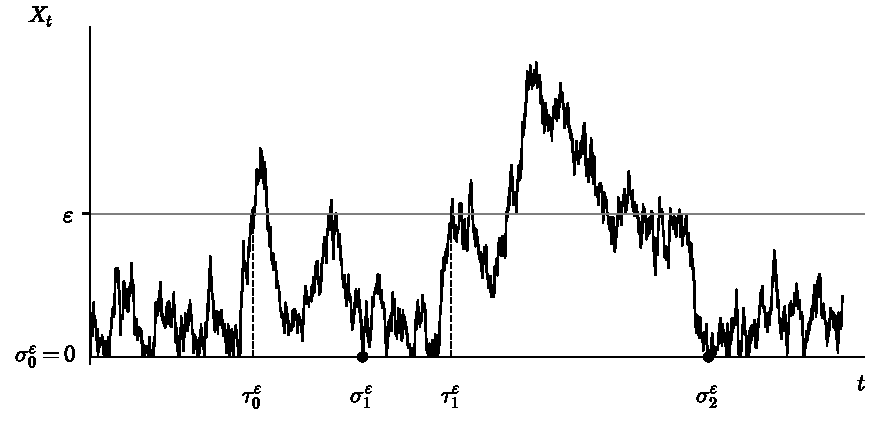
\includegraphics[width=0.8\linewidth]{figures/downcrossings.pdf}
	\caption{The stopping times defining the down-crossings from $\varepsilon$ to
		$0$, for a reflected Brownian path.}
	\label{fig1}
\end{figure}

For $p \geqslant 1$, we say that $X = M+V$ belongs to $\mathcal{S}^p$ if
\[
	\E\Big[ \langle M\rangle_\infty ^{p/2}+\Big(\int_0^\infty |dV_s|\Big)^p\Big]<\infty .
\]

\begin{theorem}\label{th:downcrossings}
	If $X = M + V$ belongs to $\mathcal{S}^p$ for some $p\geqslant 1$ and $X_0 = 0$, then
	\[
		\lim_{\varepsilon\to 0} \E\Big[\sup_{t} \Big|\varepsilon d_\varepsilon(t)-\frac{1}{2}L_t\Big|^p\Big] = 0 .
	\]
\end{theorem}

\begin{proof}
	By Tanaka's formula, for every $n$,
	\[
		X_{\tau_n\wedge t}^+ - X_{\sigma_n\wedge t}^+ =\int_{\sigma_n\wedge t}^{\tau_n\wedge t}
		1_{\{X_s >0\}}\, dX_s + \frac{1}{2}\big(L_{\tau_n\wedge t} -L_{\sigma_n\wedge t}\big) .
	\]
	Since $X$ does not vanish on $[\tau_n,\sigma_{n+1}[$, the local time $L$ is
	constant on this interval by Theorem~\ref{th3}, and summing over $n$ we obtain
	\[
		\sum_{n\geqslant 0}\big(X_{\tau_n\wedge t}^+ - X_{\sigma_n\wedge t}^+\big)
		=\int_0^t \theta_s^\varepsilon\, dX_s + \frac{1}{2}L_t,
		\qquad
		\theta_s^\varepsilon =\sum_{n\geqslant 0} 1_{]\sigma_n,\tau_n]}(s)\,1_{]0,\varepsilon]}(X_s),
	\]
	where $\theta^\varepsilon$ is predictable, with values in $\{0,1\}$. The terms
	with $\sigma_n \geqslant t$ vanish. Each $n < d_\varepsilon(t)$ satisfies
	$\tau_n \leqslant t$ and contributes $X^+_{\tau_n} - X^+_{\sigma_n} = \varepsilon$,
	while the term $n = d_\varepsilon(t)$ contributes a quantity
	$u_\varepsilon(t) \in [0,\varepsilon]$. Hence the left-hand side equals
	$\varepsilon d_\varepsilon (t)+u_\varepsilon(t)$, and the proof will be
	complete once we show that
	\[
		\lim_{\varepsilon \to 0} \E\Big[ \sup_{t}\Big| \int_0^t \theta_s^\varepsilon\, dX_s \Big|^p\Big]=0 .
	\]
	By the Burkholder--Davis--Gundy inequality, this expectation is bounded by
	\[
		C_p \E\Big[ \Big(\int_0^\infty \theta_s^\varepsilon\, d\langle M\rangle_s \Big)^{p/2}
		+ \Big(\int_0^\infty \theta_s^\varepsilon\, |dV_s| \Big)^p\Big] .
	\]
	Since $\theta^\varepsilon_s \leqslant 1_{]0,\varepsilon]}(X_s) \to 0$ for every $s$ as
	$\varepsilon\to 0$, the dominated convergence theorem, applied first to the
	inner integrals and then to the expectation (with the integrable bound
	provided by $X\in\mathcal{S}^p$), shows that this quantity tends to $0$.
\end{proof}

\section{Symmetric local times}

Let $X$ be a continuous semimartingale. Besides $\sgn$, we use the symmetric
sign function
\[
	\widehat{\sgn}(x)=1_{\{x>0\}}-1_{\{x < 0\}}, \qquad\text{so that}\qquad
	\sgn(x) = \widehat{\sgn}(x) - 1_{\{x=0\}} .
\]
Tanaka's formula can then be rewritten as
\[
	|X_t - a| =|X_0 - a| + \int_0^t \widehat{\sgn}( X_s - a)\, dX_s
	- \int_0^t 1_{\{X_s = a \}}\,dX_s + L_t^a .
\]
\begin{definition}\label{def:symlocaltime}
	The \textbf{symmetric local time} of $X$ at $a$ is
	\[
		\hat{L}_t^a = L_t^a - \int_0^t 1_{\{X_s = a \}}\,dX_s
		= \frac{L^a_t + L^{a-}_t}{2},
	\]
	where the second equality follows from Theorem~\ref{th8}.
\end{definition}
With this definition, the symmetric Tanaka formula reads
\[
	|X_t - a| =|X_0 - a| + \int_0^t \widehat{\sgn}( X_s - a)\, dX_s + \hat{L}_t^a .
\]
By Theorem~\ref{th8}, $\hat{L}^a = L^a$ when $X$ is a local martingale, and more
generally whenever $\int_0^t 1_{\{X_s=a\}}\,dV_s = 0$. The following example shows
that the two local times differ in general.

\begin{example}\label{ex:twosided}
	Let $B$ be a Brownian motion, let $c_+, c_- > 0$ and
	\[
		X_t=c_+ B_t^+ - c_- B_t^- .
	\]
	By Tanaka's formula, and since $\int_0^t 1_{\{B_s=0\}}\,dB_s =0$,
	\[
		B_t^+ = \int_0^t 1_{\{B_s >0 \}}\,dB_s + \frac{1}{2} L_t^0(B),
		\qquad
		B_t^- = -\int_0^t 1_{\{B_s <0 \}}\,dB_s + \frac{1}{2} L_t^0(B),
	\]
	hence
	\[
		X_t = \int_0^t \big(c_+1_{\{B_s >0 \}} + c_- 1_{\{B_s <0 \}}\big)\,dB_s
		+ \frac{c_+-c_-}{2} L_t^0 (B) .
	\]
	The finite variation part of $X$ is $V=\frac{c_+-c_-}{2} L^0 (B)$. Since
	$\{X_s =0 \}=\{B_s =0 \}$ and $dL^0(B)$ is carried by $\{s : B_s = 0\}$
	(Theorem~\ref{th3}), Theorem~\ref{th8} gives
	\[
		L_t^0 (X) - L_t^{0-} (X) = (c_+-c_-) \int_0^t 1_{\{B_s =0 \}}\,dL_s^0 (B) = (c_+-c_-) L_t^0 (B) .
	\]
	In fact, applying Tanaka's formula to $X^+ = c_+B^+$ and $X^- = c_-B^-$
	shows that $L^0(X) = c_+ L^0(B)$ and $L^{0-}(X) = c_- L^0(B)$, so that
	\[
		\hat{L}_t^0(X) = \frac{c_+ + c_-}{2}\, L_t^0(B) \neq L_t^0(X)
		\qquad\text{when } c_+ \neq c_- \text{ and } t > 0.
	\]
\end{example}

The argument of Corollary~\ref{cor1}, using that $x\mapsto L^x_t$ is càdlàg,
shows that almost surely, for every $a$ and $t$,
\[
	\hat{L} _t^a(X)=\lim_{\varepsilon \downarrow 0} \frac{1}{2\varepsilon}
	\int_0^t 1_{]a-\varepsilon , a+\varepsilon[}(X_s)\,d\langle X\rangle_s .
\]
We now state the It\^o--Tanaka formula in terms of symmetric local times.

\begin{theorem}[Symmetric It\^o--Tanaka formula]\label{th:symitotanaka}
	Let $X$ be a continuous semimartingale and let $f$ be the difference of two
	convex functions, with symmetric derivative
	$f'_{\mathrm{s}}=\frac{1}{2}(f'_- +f'_+)$ and with $f''=\mu$ in the sense of
	distributions. Then
	\[
		f(X_t)-f(X_0)=\int_0^t f'_{\mathrm{s}}(X_s)\,dX_s
		+ \frac{1}{2}\int_\mathbb{R} \hat{L}_t^a\, \mu (da) .
	\]
\end{theorem}

\begin{proof}
	The proof is the same as that of Theorem~\ref{th4}, with $\sgn$ replaced by
	$\widehat{\sgn}$ and Tanaka's formula replaced by its symmetric version. With
	$g(x)=\frac{1}{2}\int_{[-N,N]} |x-a|\,\mu(da)$, the symmetric derivative of
	$g$ is $g'_{\mathrm{s}}(x)=\frac{1}{2}\int_{[-N,N]} \widehat{\sgn}(x-a)\,\mu(da)$,
	since the symmetric derivative of $|x-a|$ is $\widehat{\sgn}(x-a)$.
	Integrating the symmetric Tanaka formula with respect to
	$\frac{1}{2}\mu(da)$ and applying Theorem~\ref{th5} gives
	\[
		g(X_t)-g(X_0)= \int_0^t g'_{\mathrm{s}}(X_s)\,dX_s
		+ \frac{1}{2} \int_{[-N,N]} \hat{L}_t^a\,\mu(da),
	\]
	and $\hat{L}_t^a=0$ for $|a| > N$, which completes the proof.
\end{proof}
